\documentclass[12pt,letterpaper]{article}
\usepackage{fullpage}
\usepackage[top=2cm, bottom=4.5cm, left=2.5cm, right=2.5cm]{geometry}
\usepackage{amsmath,amsthm,amsfonts,amssymb,amscd}
\usepackage{lastpage}
\usepackage{enumerate}
\usepackage{fancyhdr}
\usepackage{mathrsfs}
\usepackage{xcolor}
\usepackage{graphicx}
\usepackage{svg}
\usepackage{listings}
\usepackage[bookmarksopen=true]{hyperref}
\usepackage[yyyymmdd]{datetime}
\usepackage[open]{bookmark}

\hypersetup{%
  colorlinks=true,
  linkcolor=blue,
  linkbordercolor={0 0 1}
}
 
\renewcommand\lstlistingname{Algorithm}
\renewcommand\lstlistlistingname{Algorithms}
\def\lstlistingautorefname{Alg.}

\lstdefinestyle{Python}{
    language        = Python,
    frame           = lines, 
    basicstyle      = \footnotesize,
    keywordstyle    = \color{blue},
    stringstyle     = \color{green},
    commentstyle    = \color{red}\ttfamily
}

\setlength{\parindent}{0.0in}
\setlength{\parskip}{0.05in}

\newcommand\doctitle{HPGO}
\newcommand\ID{\href{https://rongyi.io}{rongyi.io}}


\pagestyle{fancyplain}
\headheight 35pt
\lhead{\ID}
\chead{\textbf{\doctitle}}
\rhead{\today}
\lfoot{DRAFT VERSION}
\cfoot{}
\rfoot{\small\thepage}
\headsep 1.5em

\begin{document}

\section{Introduction}


\texttt{\textcolor{blue}{
\quad \textcolor{gray}{LER0ever} \textcolor{red}{Internal Ref} \\
\newline
\begin{tabular}{rl}
%\texttt{\textcolor{blue}{ 
Task ID: & CU\#2672zg \\
CUT Link: & ry.sb/cut/2672zg \\
Notion: & ry.sb/n/by-f4bcf0106acc40d88e62a2e7673b229f \\
Draft: & internal.ry.sb/HPGO	
%}}
\end{tabular}
}}


\section {Notations}
\subsection {Profiling}
\begin{itemize}
	\item $L$: the total number of layers
	\item $l$: the \# of a layer, from $1$ to $L$
	\item $t_l$: "the total computation time across the forward and backward passes for layer l on the target GPU"
	\item $a_l$: "the size of the output activations of layer $l$ (and the size of input gradients in the backward pass) in bytes"
	\item $w_l$: "the size of weight parameters for layer $l$ in bytes"
	\item $A(i \rightarrow j)$
	\item $PBS$: Profiling Batch Size
\end{itemize}
\subsection {Model}
\begin{itemize}
	\item $GBS$: the Global Batch Size for training
	\item (optional) $allow\_async$: if the model can be trained in a non-BSP fashion.
\end{itemize}
\subsection {Environment}
\begin{itemize}
	\item $M$: number of Workers (GPUs) in total
	\item $m$: the \# of a worker, from $1$ to $M$
	\item $B_{i \rightarrow j}$ Theoretical Bandwidth limit from worker $i$ to worker $j$
	\item $B(i,j,b)$: estimated actual bandwidth from worker $i$ to worker $j$, transferring $b$ bytes of data (normally an S curve)
\end{itemize}
\subsection {HPGO Result}
\begin{itemize}
	\item $S$: the model is partitioned into $S$ stages
	\item $R_s$: for stage $s$  $(0 \le s < S)$, it is replicated $R_s$ times using Split-Concat
	\item $R_P$: the number of Pipelines in the outermost Data Parallel
	\item $L_s = \{...\}$: all the consecutive layers in stage $s$
	\item $T_s$: the total computational time for stage $s$, calculated as $\sum_{l \in L_s} {t_l}$
	\item $A_s$: the total activation output for stage $s$, calculated as the activation for the last layer in that stage
	\item $W_s$: the total parameter size for stage $s$, calculated as $\sum_{l \in L_s} w_l$
	\item $B_{s \rightarrow t}(b)$: Bandwidth from stage $s$ to a connecting stage $t$, sending $b$ bytes of data. This is estimated by the inter-worker bandwidth of where those two stages are on, as well as a theoretical estimation of the real bandwidth it can achieve with $b$ bytes of data.

\end{itemize}

\section {Parallelism}
Given an arbitrary model, the algorithm will try to partition the model into different distinct stages. Those stages can then be replicated to make sure the pipeline won't be slowed down by stragglers. And we then replicate the entire pipeline to scale further if needed. 

Replicated Stages inside a pipeline are implemented in a Split-Concat fashion, where the original input tensors are splitted before the stage and concatted afterwards. 

Replicated Pipelines are achieved through traditional Data Parallelism, with each stages of the pipeline synchronizing their weights independently.

\subsection {Split-Concat}
This happens when the $i$-th stage needs to receive data (mainly activations) from the previous stage ($i-1$)th. 

Assume the $i$-th stage has $m_i$ workers and the ($i-1$)th stage has $m_{i-1}$ workers. Then the size of activations needed to be transfer is the same as the same stage with no replica. 

So if every worker of stage $i-1$  has the same inter-worker bandwidth with any of those of stage $i$, the time estimated to transfer the activations is $A_{s-1} / B_{i-1 \to i}(A_{s-1})$

On the other hand if the bandwidth between these two stages are not uniform, we can still calculate the estimated transfer time by tracing the communication route between any two workers.
We know that the $R_{i-1}$ workers of stage ($i-1$) need to transfer $A_{s-1}$ bytes of data to $R_i$ workers of stage $i$, this is normally achieved by splitting the original Activation tensors into $R_i$ pieces on each of the $R_{i-1}$ workers. So the overall estimated transfer time should be 
$$max_{x=0}^{R_{i-1}}\ max_{y=0}^{R_i}\ \left\{\begin{array}{lr}
        	\frac{(A_{s-1}/(R_{i-1} \times R_i))}{B_{x \to y}(A_{s-1}/(R_{i-1} \times R_i))}
        \end{array}\right\}$$
In the real-world scenario with 2-level networking setup (one being inter-machine ethernet, the other being NVLink within machines), this is essentially the time taken by transferring one of the above slice through ethernet, as transferring the same size of data through NVLink is several magnitudes faster: 
$$(A_{s-1}/(R_{i-1} \times R_i)) / B_{eth}(A_{s-1}/(R_{i-1}\times R_i))$$

\subsection {Data Parallelism}
Data Parallelism is used only at the very outer level of system to further scale the pipelines. Each stage in the inner pipeline does DP AllReduce with the same stage of all other pipelines. Let's say we have a 8 stage pipeline, extended with DP 8 times, then stage 1 of each pipeline do AllReduce's together. 

All the AllReduce operations are deferred to the very end of each pipeline, after all the micro-batches in the pipeline. This is similar to what one would get from Gradient Accumulation. The amount of parameters needed to do a single AllReduce is equal to all the weights combined in that stage: $W_s = \sum_{l \in L_s} w_l$

Therefore the total weights needed to communicate is $\frac{2*W_s * (R_P-1)}{R_P}$, yielding the estimated time for doing one AllReduce operation is
$$\frac{2 \times W_s \times (R_P-1)}{R_P \times B_{slowest}(2 \times W_s \times  \frac{R_P-1}{R_P})}$$
where we take the slowest network bandwidth across all the AllReduce nodes for time estimation. 


\subsection {Synchronous Pipeline}
\subsubsection {Synchronous Pipeline, where networks are negligible}

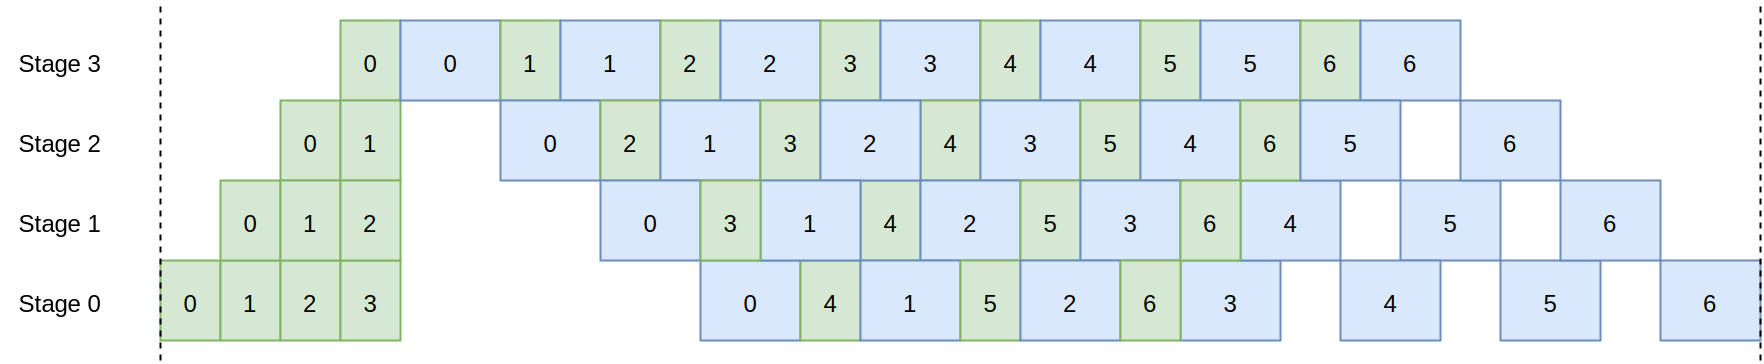
\includegraphics[width=\textwidth]{../images/HPGO-Pipeline-no-network.png}

\subsubsection {Synchronous Pipeline, where networks are likely to be bottlenecks}

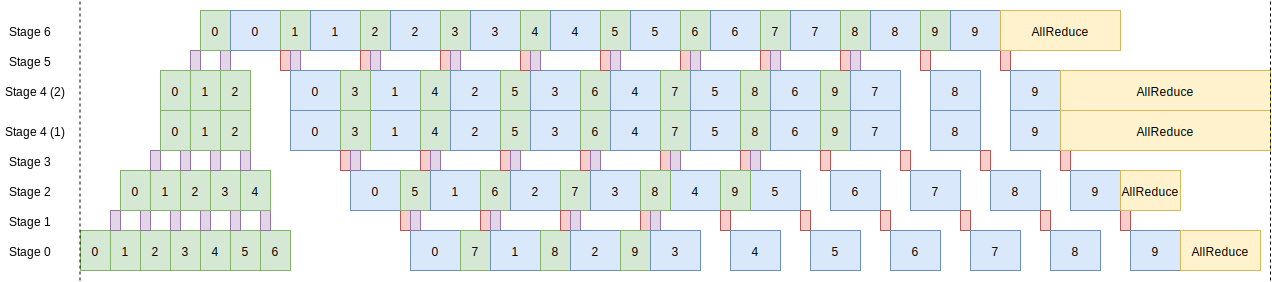
\includegraphics[width=\textwidth]{../images/HPGO-Pipeline.png}

\subsubsection{Efficiency}
Pipeline Length:
\begin{gather}
	$$PL = \max_{0 \le i < S,\ i\ \%\ 2 == 0} \\\{
        	(mbatch \times (fw[q] + bw[q]) + \sum_{k=0}^{q-1}{(fw[k] + bw[k])}) \\- \sum_{s=0}^i bw[s] + \frac{2 \times w_i \times (r_p-1)}{r_p \times b_{slowest}(2 \times w_i \times \frac{r_p-1}{r_p})} \}$$
\end{gather}
Actual Computation Blocks: 
$$CB = \sum_{0 \le i < S,\ i\ \%\ 2 == 0} mBatch \times (FW[i] + BW[i])$$

Overall Pipeline Efficiency for Speedup Calculation:
$$\frac{CB}{PL * \lceil S / 2 \rceil}$$
\subsection {Asynchronous Pipeline}
\texttt{\textcolor{blue}{
\quad \textcolor{gray}{LER0ever} \textcolor{red}{Internal Ref} \\
\newline
\begin{tabular}{rl}
%\texttt{\textcolor{blue}{ 
Task ID: & CU\#2672zg \\
Copybara: & Disabled for ENV \$ ry.hg/UX9Q/HPGO/DAPPLE	
%}}
\end{tabular}
}}

\subsection {Hybrid Parallelism}

\section {HPGO v0.7}

The following subsections describe the algorithm in a progressive manner, from the one that was simplified to the extreme, to the full Orchestration algorithm able to optimize real-world training situations.

\subsection{Var.1: Asynchronous, No-Replication, No-Networks, No-Placement}

Assume the following to simplify the problem to the extreme:
\begin{enumerate}
	\item the pipeline runs forever without needing to synchronize
	\item we do not have any replication whatsoever
	\item communications are negligible compared to computations
	\item once the split is determined, we magically have the optimal placement
	\item we only have one pipeline, without any outer DP.
\end{enumerate}

\subsubsection{Problem Reduction}

then essentially we want to the the following problem:

\begin{quote}
	Given a model and its profiling results, along with the number of workers, what's the best way to partition the model so that \textbf{the pipeline runs the fastest}?
\end{quote}

This problem can then be further reduced to:

\begin{quote}
	Given a model and its profiling results, along with the number of workers, what's the best way to partition the model so that the \textbf{slowest stage in the pipeline is the fastest}?
\end{quote}

Define the number of stages as $n$ and the number of workers as $k$, this problem is then equivalent to:

\begin{quote}
	Given an array of $n$ numbers, find a partition solution so that the array is splitted into $k$ parts, and the maximum of the $k$ sums (by adding elements of each subarray together) is minimized.
\end{quote}

\subsubsection{Solution to this problem}
The brutal force solution to this problem has the time complexity of $O(n^k)$, and the best solution using binary search can get us down to $O(n log(sum(A)))$.

But for the ease of outputing the actual partition solution, we use Dynamic Programming to solve this problem:

Define \texttt{dp[i][j]} as the slowest stage time when splitting the first $i+1$ layers into $j$ stages, assuming the split is already optimal.

If we look at the $j$-th stage in that equation, we can iterate the starting layer ID of that stage to make sure we get the optimal $j$-th stage, that is: $max_{p=0}^{i}(dp[p][j-1], A[p+1] + ... + A[i]$. This means that the slowest stage up to the $j$-th can be expressed as the slowest stage among the first $j-1$ stages and the $j$-th stage itself. 

Define the state transition function as follows:

\texttt{dp[i][j] = $min$\{$max_{p=0}^{i}$\{dp[i][1]-dp[p][1],dp[p][j-1]\}\}}

And we can get the solution by solving \texttt{dp[n][k]}.

$$dp[n][k] = \min_{i=1}^n\{\min_{j=1}^k\{\max_{p=0}^i\{dp[i][1]-dp[p][1],dp[p][j-1]\}\}\}$$

\subsubsection{Space-Time Complexity}
This DP-based solution has the time complexity of $O(n^2*k)$ and the space complexity of $O(n*k)$.
 
\subsection{Var.2: Asynchronous, No-Networks, No-Placement}
We loosen the constraints on replication, but still assume the following:
\begin{enumerate}
	\item the pipeline runs forever without needing to synchronize
	\item communications are negligible compared to computations
	\item once the split is determined, we magically have the optimal placement
	\item we only have one pipeline, without any outer DP.
\end{enumerate}

This time certain stages are allowed to be replicated so that the compute time can be reduced linearly. 

\subsubsection{Problem Reduction}
Restate the problem:
\begin{quote}
	Given a model and its profiling results, along with the number of workers, what's the best way to partition the model into stages and optionally replicate certain stages, so that the \textbf{slowest stage in the pipeline is the fastest}?
\end{quote}

Define the number of stages as $n$ and the number of workers as $k$, this problem is equivalent to:
\begin{quote}
	Given an array of $n$ numbers, find a partition so that the array is splitted into $m$ parts ($m \le k$), and assume each subarray has a weight of a natural number such that the weights of all subarrays added together is $k$. We add each subarray elements to get $m$ sums, find the solution when the maximum of those $m$ sums is minimized.
\end{quote}

\subsubsection{Solution to this problem}
This problem is different from the last one in a sense that the split is not necessarily $k$. So the original brute force solution still work in exponential time, but the binary search solution in $O(n*k)$ will no longer work.

Here I propose a slightly modified DP solution, where it simultaneously explore on how to partition the model as well as how many replicas per stage.

Define \texttt{dp[i][j]} as the slowest stage time when splitting the first $i+1$ layers into stages with $j$ machines, assuming the split is already optimal.

Consider the last stage in dp[i][j], where we can either shift its starting point $i'$ or tweaking the number of workers allocated to that stage $j'$, therefore it can be expressed as the following state transition function:

$$dp[i][j] = \min_{0<i'<i}\min_{0<j'<j}\ \max\ \left\{\begin{array}{lr}
        	\frac{dp[i][1] - dp[i'][1]}{j'} \\
        	dp[i'][j-j']
        \end{array} \right .$$
        
Thus solving for dp[n][k] would give us the answer:

$$dp[n][k] = \min_{i=1}^n\min_{j=1}^k\min_{0<i'<i}\min_{0<j'<j}\ \max\ \left\{\begin{array}{lr}
        	\frac{dp[i][1] - dp[i'][1]}{j'} \\
        	dp[i'][j-j']
        \end{array} \right .$$

\subsubsection{Space-Time Complexity}
This solution has the time complexity of $O(n^2k^2)$, and the space complexity of $O(n * k)$.

\subsection{Var.3: Asynchronous, No-Placement}
We added the constraints on networks, but still assume the following:
\begin{enumerate}
	\item the pipeline runs forever without needing to synchronize
	\item once the split is determined, we magically have the optimal placement
	\item we only have one pipeline, without any outer DP.
\end{enumerate}

This problem is now similar to what the PipeDream's Optimizer tries to solve.

For each stage, there is an input to that stage needed to be performed before the computation could even start, and an output generated for the next stage which can be overlapped with the next round of computation. 
% Therefore, it makes the most sense to put the input data transmission together with the main computation as a whole. 

For stages with replications, the calculation for the communication is mentioned at \hyperref[sec:Split-Concat]{Split-Concat}.

\subsubsection{Problem Reduction}

We still define the number of stages as $n$ and the number of workers as $k$. Assume computation for each stage is $C[]$, and activation input and output are $A_i[]$ and $A_o[]$. This problem is then equivalent to:

\begin{quote}
	Given an array of $n$ numbers, find a partition so that the array is splitted into $m$ parts ($m \le k$), and assume each subarray has a weight of a natural number such that the weights of all subarrays added together is $k$. For each elements in the array, the value is then recalculated to be the largest among computation times and communication time, and then we add each subarray elements to get $m$ sums. Find the solution when the maximum of those $m$ sums is minimized.
\end{quote}

\subsubsection{Solution to this problem}
The DP approach to solve this is similar to the last solution, except that we need to take the max of current stage computation time, current stage input/output time, and previous split optimal time. We further simplify the problem by assuming Half Duplexing.

So the state transition function then becomes:
$$dp[i][j] = \min_{0<i'<i}\min_{0<j'<j}\ \max\ \left\{\begin{array}{lr}
        	\frac{dp[i][1] - dp[i'][1]}{j'} \\
        	dp[i'][j-j'] \\
        	A_i[i'] + A_o[i']
        \end{array} \right .$$
        
The answer to this is therefore:

$$dp[n][k] = \min_{i=1}^n\min_{j=1}^k\min_{0<i'<i}\min_{0<j'<j}\ \max\ \left\{\begin{array}{lr}
        	\frac{dp[i][1] - dp[i'][1]}{j'} \\
        	dp[i'][j-j'] \\
        	A_i[i'] + A_o[i']
        \end{array} \right .$$
        
\subsubsection{Space-Time Complexity}
This solution has the time complexity of $O(n^2k^2)$, and the space complexity of $O(n * k)$.

\subsection{Var.4: Synchronous, No-Placement, No-Network}
We now enforce strictly synchronous training, but still assume the following:
\begin{enumerate}
	\item communications are negligible compared to computations
	\item once the split is determined, we magically have the optimal placement
	\item we only have one pipeline, without any outer DP.
\end{enumerate}


For Synchronous Pipeline, we arrange the forward/backward computation of a model in a deterministic way to minimize peak activation memory. 

The length of a single synchronous pipeline is estimated by the following formula, assuming stage Q is the one taking the longest time (meaning "$\arg \max_i {(FW[i] + BW[i])} = Q$"):

$$mBatch \times (FW[Q] + BW[Q]) + \sum_{k=0}^{Q-1}{(FW[k] + BW[k])} $$

If we have multiple candidates for Q, we pick the one with the largest index.

\subsubsection{Problem Reduction}
In order to minimize the overall running time of the pipeline, we just need to minimize the forward and backward computation time of Q, the longest stage in the pipeline. 

This is therefore equivalent to "Var.2: Asynchronous, No-Networks, No-Placement".

\subsubsection{Solution to this problem}
Same as Var.2

$$dp[n][k] = \min_{i=1}^n\min_{j=1}^k\min_{0<i'<i}\min_{0<j'<j}\ \max\ \left\{\begin{array}{lr}
        	\frac{dp[i][1] - dp[i'][1]}{j'} \\
        	dp[i'][j-j']
        \end{array} \right .$$

\subsubsection{Space-Time Complexity}
This solution has the time complexity of $O(n^2k^2)$, and the space complexity of $O(n * k)$.

\subsection{Var.5: Synchronous, No-Placement}
For synchronous pipeline where network could potentially be a bottleneck, we arrange the network as if it's a separate stage independent from computation, as mentioned in Section 3.3 .

Without taking micro batch count into consideration, this is essentially the same as the solution for Var.4


\subsection{Var.6: Synchronous, No-Placement, DP Extension}
For an almost complete system with Data Parallel extending the inner Synchronous Pipeline, we use the same method to arrange the optimal pipeline as mentioned in Var.4 and Var.5.

Since assigning different number of available workers to a pipeline drastically affect the pipeline arrangement, we have to enumerate all the possible DP solution up to $\lceil\sqrt{n}\rceil$.

The AllReduce operation needed for Data Parallel can start immediately after a stage has done its final backward computation. In terms of pipeline length, this would only add the time for AllReduce of stage 0 in best scenario. However, it is possible for AllReduce operations from other stages to block the finishing time of the entire pipeline.

The general calculation formula for Pipeline length with DP extension is as follows, assuming stage Q is the longest stage:

\begin{gather}
	\max_{0 \le i < S,\ i\ \%\ 2 == 0} \\\{
        	(mBatch \times (FW[Q] + BW[Q]) + \sum_{k=0}^{Q-1}{(FW[k] + BW[k])}) \\- \sum_{s=0}^i BW[s] + \frac{2 \times W_i \times (R_P-1)}{R_P \times B_{slowest}(2 \times W_i \times \frac{R_P-1}{R_P})} \}
\end{gather}

(1) takes the max across all the stages, and the $i \% 2$ is to filter out network stage \\
(2) calculates the original pipeline length without AllReduce \\
(3) normalizes to when the stage actually ends, and adds the AllReduce cost

While enumerating the possible configurations for DP extension, we first arrange the entire model without considering any DP extension with all the $k$ machines, and get a theoretical max speedup over single machine $sp$, and use this as a threshold for whether we will plan for certain configurations that does not use all the machines. 

For example, if we have 16 workers available, and the single pipeline can achieve the speedup of 15.1, then we can safely abandon the 3x5 configuration as its theoretical speedup limit is 15.

For every DP configuration we try out, we also explore for its "transposed" configuration, meaning we will try 3x5 and 5x3 at the same time. 

This solution has the time complexity of $O(n^2\times k^2\times \sqrt{k})$, and the space complexity of $O(n \times k \times \sqrt{k})$.

\subsection{Var.7: Synchronous, BF Placement, DP Extension}
Once we have the placement for each stage, we only need to solve the subproblem stated in Var.6. Here we experiment on Brute Force Placement.

\subsubsection{Placement!}
This is the complexity of a Naive Brute Force $$\prod_{i=0}^s {(k - \sum_{j=0}^i {R_j}) \choose R_i} = \prod_{i=0}^s \frac{(k - \sum_{j=0}^i {R_j})!}{R_i ! \times (k - (\sum_{j=0}^i {R_j}) - R_i)!}$$

We can do better by assuming that every machine is equivalent and every graphics card inside a machine is equivalent, i.e. the entire system is composed of isomorphic components. If we have a cluster of M machines each with G graphics card, we can then cut the complexity down by at least $M! \times G!$, where $M\times G = k$.

\subsubsection{Space-Time Complexity}
This placement alone has the time complexity of 
$$BFF = O(\frac{\prod_{i=0}^s \frac{(k - \sum_{j=0}^i {R_j})!}{R_i ! \times (k - (\sum_{j=0}^i {R_j}) - R_i)!}}{k \times (M-1)!(G-1)!})$$

For each enumeration of placement, we need to store all the DP states in order to get the best solution. Therefore the space complexity compared to Var.6 is $BFF$ times larger.

\subsection{Var.8: Synchronous, Placement Heuristics, DP Extension}
In our use cases, if we have a stage with more than 1 replica, the AllReduce speed can be estimated using the lowest bandwidth across these replicas, same for the calculation of Activation communication. Therefore, it is sufficient to consider device placement as the following three cases:
\begin{enumerate}
	\item \textbf{FF}(Fresh First): prioritize placing the entire stage on a fresh unused machine
	\item \textbf{AF}(Append First): prioritize placing the entire stage after an existing stage on a not yet fully occupied machine, even if this means the stage has to cross multiple machines
	\item \textbf{GF}(Gaps First): prioritize filling in the gaps on machines not yet fully utilized
\end{enumerate}

This would significantly cut down the space and time complexity to enumerate all the possible placement of stages. Assume we have $M$ machines each with $G$ graphics card, $M \times G = k$, then the total complexity for this process is strictly less than:
$$O((2\times M)^s)$$

Along with DP extension enumeration and Device Rotation, the overall complexity without Single Pipeline Arrangement, is strictly less than:

$$O(\sum_{i=0}^{\lceil \sqrt{k} \rceil} (2 \times (\lceil M/i \rceil))^i)$$

Therefore the total complexity for this improved enum-based approach is
$$O(n^2 \times k^2 \times \sum_{i=0}^{\lceil \sqrt{k} \rceil} (2 \times (\lceil M/i \rceil))^i)$$

\subsection {The Full Algorithm}
\subsubsection{Max-Flow Min-Cut with Dynamic Trees (Dinic's)}

\subsubsection{Device Rotation}

\subsubsection{Single Pipeline Arrangement}

\subsubsection{DP Extension Enumeration}

\subsection {Proof of Correctness}

\subsection {Complexity Analysis}

$\downarrow$ Draft $\downarrow$
\subsubsection* {First attempt: 
$O(|B|^2M^2N^4)$}
This attempt ignored batch size information and device memory
\subsubsection* {Second attempt:
$\Theta(M!M^2N^4|B|^2)$}
Use a Max-Flow based algorithm to perform Single Pipeline Partitioning.
\subsubsection* {Third attempt:
$\Theta(M!Mlog(M)N^4|B|^2)$}
Use a Dynamic Tree based Max-Flow for arranging SPP.

\subsubsection* {PipeDream: $\sum_{k=1}^L O(N^3m_k^2)$}

\end{document}
